\documentclass{beamer}
\usepackage[utf8]{inputenc}
\usepackage{graphicx, epsfig}
\usepackage{amsmath,mathrsfs,amsfonts,amssymb}
\usepackage{floatflt}
\usepackage{epic,ecltree}
\usepackage{mathtext}
\usepackage{fancybox}
\usepackage{fancyhdr}
\usepackage{multirow}
\usepackage{enumerate}
\usepackage{epstopdf}
\usepackage{multicol}
\usepackage{algorithm}
\usepackage[noend]{algorithmic}
\usepackage{tikz}
\usepackage{blindtext}
\usepackage{multido}
\usetheme{default}%{Singapore}%{Warsaw}%{Warsaw}%{Darmstadt}
\usecolortheme{default}

\setbeamerfont{title}{size=\Huge}
\setbeamertemplate{footline}[frame number]{}

\setbeamertemplate{section in toc}[sections numbered]

\makeatletter
\newcommand\HUGE{\@setfontsize\Huge{35}{40}}
\makeatother    

\setbeamerfont{title}{size=\HUGE}
\beamertemplatenavigationsymbolsempty

\usetikzlibrary{arrows,shapes,positioning,shadows,trees}

\newcommand\myfootnote[1]{%
  \vspace{-0.5cm}%
  \tikz[remember picture,overlay]
  \draw (current page.south west) +(1in + \oddsidemargin,0.5em)
  node[anchor=south west,inner sep=0pt]{\parbox{\textwidth}{%
      \rlap{\rule{10em}{0.4pt}}\raggedright\scriptsize \textit{#1}}};}

\newcommand\myfootnotewithlink[2]{%
  \vspace{-0.5cm}%
  \tikz[remember picture,overlay]
  \draw (current page.south west) +(1in + \oddsidemargin,0.5em)
  node[anchor=south west,inner sep=0pt]{\parbox{\textwidth}{%
      \rlap{\rule{10em}{0.4pt}}\raggedright\scriptsize\href{#1}{\textit{#2}}}};}

\AtBeginSection[]
      {
      	\begin{frame}{Outline}
      		\tableofcontents[currentsection]
      	\end{frame}
      }
      \AtBeginSubsection[]{
      	\begin{frame}{Outline}
      		\tableofcontents[currentsection,currentsubsection]
      	\end{frame}
}

\newcounter{noscounter} % Используется для nextonslide команды (обнуляется только на новом слайде)
\newcounter{pcounter} % Используется для pause команды (обнуляется после использования eqpause)
\newcounter{diffcounter} % Считает количество pause после формулы

\newcommand{\nextonslide}[1]{%
  \stepcounter{noscounter}% Прибавляем счетчик nextonslide
  \stepcounter{pcounter}% Прибавляем счетчик pause
  \stepcounter{diffcounter}% Прибавляем счетчик diffcounter
  \onslide<\value{noscounter}->{#1}% Отображаем аргумент в скобках на слайде с номером noscounter
}
\newcommand{\resetonslide}{%
    \setcounter{noscounter}{1}% Сбрасываем счетчик nextonslide
    \setcounter{pcounter}{1}% Сбрасываем счетчик pause
    \setcounter{diffcounter}{0}% Сбрасываем счетчик diffcounter
}

\newcommand{\eqpause}{%
  \multido{\i=1+1}{\value{pcounter}}{\pause}% Повторяем pcounter раз команду pause
  \stepcounter{noscounter}% Прибавляем счетчик nextonslide
  \setcounter{pcounter}{1}% Сбрасываем счетчик pause
}

\newcommand{\eqpausediff}{% Вспомогательная команда, запускается автоматически после формул
  \multido{\i=1+1}{\value{diffcounter}}{\pause}% Повторяем diffcounter раз команду pause
  \addtocounter{pcounter}{-\value{diffcounter}}% Вычитаем из pcounter количество сделанных pause
  \setcounter{diffcounter}{0}% Сбрасываем счетчик diffcounter
}

\newcommand\AtEndBoth[2]{% Применяем команду к multline и multline*
  \AtEndEnvironment{#1}{#2}%
  \AtEndEnvironment{#1*}{#2}%
}

\AtEndBoth{align}{\eqpausediff}
\AtEndBoth{equation}{\eqpausediff}
\AtEndBoth{multline}{\eqpausediff}

\addtobeamertemplate{frametitle}{\resetonslide}{}% На каждом слайде сбрасываем счетчики

% latin bold lower
\newcommand{\ba}{\mathbf{a}} 
\newcommand{\bc}{\mathbf{c}} 
\newcommand{\be}{\mathbf{e}} 
\newcommand{\bff}{\mathbf{f}} % \bf - for bold type
\newcommand{\bg}{\mathbf{g}} 
\newcommand{\bh}{\mathbf{h}} 
\newcommand{\bp}{\mathbf{p}} 
\newcommand{\bq}{\mathbf{q}} 
\newcommand{\bt}{\mathbf{t}} 
\newcommand{\bs}{\mathbf{s}} 
\newcommand{\bu}{\mathbf{u}} 
\newcommand{\bv}{\mathbf{v}} 
\newcommand{\bw}{\mathbf{w}} 
\newcommand{\bx}{\mathbf{x}} 
\newcommand{\by}{\mathbf{y}} 
\newcommand{\bz}{\mathbf{z}} 

% latin bold upper
\newcommand{\bA}{\mathbf{A}} 
\newcommand{\bB}{\mathbf{B}} 
\newcommand{\bC}{\mathbf{C}} 
\newcommand{\bG}{\mathbf{G}} 
\newcommand{\bI}{\mathbf{I}} 
\newcommand{\bJ}{\mathbf{J}} 
\newcommand{\bL}{\mathbf{L}} 
\newcommand{\bM}{\mathbf{M}} 
\newcommand{\bP}{\mathbf{P}}
\newcommand{\bQ}{\mathbf{Q}} 
\newcommand{\bR}{\mathbf{R}} 
\newcommand{\bT}{\mathbf{T}} 
\newcommand{\bU}{\mathbf{U}} 
\newcommand{\bV}{\mathbf{V}} 
\newcommand{\bW}{\mathbf{W}} 
\newcommand{\bX}{\mathbf{X}} 
\newcommand{\bY}{\mathbf{Y}} 
\newcommand{\bZ}{\mathbf{Z}} 

% latin cal upper
\newcommand{\cF}{\mathcal{F}} 
\newcommand{\cG}{\mathcal{G}} 
\newcommand{\cI}{\mathcal{I}} 
\newcommand{\cL}{\mathcal{L}} 
\newcommand{\cM}{\mathcal{M}} 
\newcommand{\cN}{\mathcal{N}} 
\newcommand{\cP}{\mathcal{P}} 
\newcommand{\cS}{\mathcal{S}} 
\newcommand{\cT}{\mathcal{T}} 
\newcommand{\cW}{\mathcal{W}} 
\newcommand{\cX}{\mathcal{X}} 
\newcommand{\cZ}{\mathcal{Z}} 

% latin bb upper
\newcommand{\bbE}{\mathbb{E}} 
\newcommand{\bbI}{\mathbb{I}} 
\newcommand{\bbP}{\mathbb{P}} 
\newcommand{\bbR}{\mathbb{R}} 

% greek bold lower
\newcommand{\bepsilon}{\boldsymbol{\epsilon}} 
\newcommand{\btheta}{\boldsymbol{\theta}} 
\newcommand{\blambda}{\boldsymbol{\lambda}} 
\newcommand{\bpi}{\boldsymbol{\pi}} 
\newcommand{\bmu}{\boldsymbol{\mu}} 
\newcommand{\bsigma}{\boldsymbol{\sigma}} 
\newcommand{\bphi}{\boldsymbol{\phi}} 

% greek bold upper
\newcommand{\bSigma}{\boldsymbol{\Sigma}} 

\DeclareMathOperator*{\argmin}{arg\,min}
\DeclareMathOperator*{\argmax}{arg\,max}
\newcommand{\createdgmtitle}[1]{\title[\hbox to 56mm{Deep Generative Models  \hfill\insertframenumber\,/\,\inserttotalframenumber}]
	{\vspace{1cm} \\ \textbf{Deep Generative Models} \\ {\Huge Lecture #1}}
	\author{Roman Isachenko}
	\institute{
		Moscow Institute of Physics and Technology \\
		Yandex School of Data Analysis
	}
	\date{2025, Autumn}
}
\createdgmtitle{4}
%--------------------------------------------------------------------------------
\begin{document}
%--------------------------------------------------------------------------------
\begin{frame}[noframenumbering,plain]
	\titlepage
	\resetonslide
\end{frame}
%=======
\begin{frame}{Recap of Previous Lecture}
	\begin{block}{Latent Variable Models (LVM)}
		\vspace{-0.3cm}
		\[
			\pt(\bx) = \int \pt(\bx, \bz) d\bz = \int \pt(\bx | \bz) p(\bz) d\bz.
		\]
	\end{block}
	\begin{block}{MLE Problem for LVM}
		\vspace{-0.7cm}
		\begin{multline*}
			\btheta^* = \argmax_{\btheta} \log \pt(\bX) = \argmax_{\btheta} \sum_{i=1}^n \log \pt(\bx_i) = \\ = \argmax_{\btheta}  \sum_{i=1}^n \log \int \pt(\bx_i| \bz_i) p(\bz_i) d\bz_i.
		\end{multline*}
		\vspace{-0.7cm}
	\end{block}
	\begin{block}{Naive Monte Carlo Estimation}
		\vspace{-0.7cm}
		\[
			\pt(\bx) = \int \pt(\bx | \bz) p(\bz) d\bz = \bbE_{p(\bz)} \pt(\bx | \bz) \approx \frac{1}{K} \sum_{k=1}^{K} \pt(\bx | \bz_k),
		\]
		\vspace{-0.5cm} \\
		where $\bz_k \sim p(\bz)$. 
	\end{block}
\end{frame}
%=======
\begin{frame}{Recap of Previous Lecture}
	\begin{block}{ELBO Derivation 1 (Inequality)}
		\[
			\log \pt(\bx) = \log \int \pt(\bx, \bz) d\bz \geq \bbE_{q} \log \frac{\pt(\bx, \bz)}{q(\bz)} = \cL_{q, \btheta}(\bx)
		\]
		\vspace{-0.3cm}
	\end{block}
	\begin{block}{ELBO Derivation 2 (Equality)}
		\vspace{-0.3cm}
		\begin{multline*}
			\cL_{q, \btheta}(\bx) = \int q(\bz) \log \frac{\pt(\bx, \bz)}{q(\bz)}d\bz = 
			\int q(\bz) \log \frac{\pt(\bz|\bx)\pt(\bx)}{q(\bz)}d\bz = \\
			= \log \pt(\bx) - \KL(q(\bz) \| \pt(\bz|\bx))
		\end{multline*}
	\end{block}
	\vspace{-0.3cm}
	\begin{block}{Variational Decomposition}
		\[
		\log \pt(\bx) = \cL_{q, \btheta}(\bx) + \KL(q(\bz) \| \pt(\bz|\bx)) \geq \cL_{q, \btheta}(\bx).
		\]
	\end{block}
\end{frame}
%=======
\begin{frame}{Recap of Previous Lecture}
	\begin{block}{Variational Evidence Lower Bound (ELBO)}
		\vspace{-0.3cm}
		\[
			\log \pt(\bx) = \cL_{q, \btheta}(\bx) + \KL(q(\bz) \| \pt(\bz|\bx)) \geq \cL_{q, \btheta}(\bx).
		\]
	\end{block}

	\vspace{-0.5cm}
	\[
	 	{\color{olive}\cL_{q, \btheta}(\bx)} = \int q(\bz) \log \frac{\pt(\bx, \bz)}{q(\bz)}d\bz = \bbE_{q} \log \pt(\bx | \bz) - \KL (q(\bz) \| p(\bz))
	\]
	\vspace{-0.3cm}
	\begin{block}{Log-likelihood Decomposition}
		\vspace{-0.5cm}
		\[
	 		\log \pt(\bx) = {\color{olive}\bbE_{q} \log \pt(\bx | \bz) - \KL (q(\bz) \| p(\bz))} + \KL(q(\bz) \| \pt(\bz|\bx)).
		\]
	\end{block}
	\begin{itemize}
		\item Rather than maximizing likelihood, maximize the ELBO:
		\[
			\max_{\btheta} \pt(\bx) \quad \rightarrow \quad \max_{q, \btheta} \cL_{q, \btheta}(\bx)
		\]
		\item Maximizing the ELBO with respect to the variational distribution $q$ is equivalent to minimizing the KL divergence:
		\[
			\argmax_q \cL_{q, \btheta}(\bx) \equiv \argmin_q \KL(q(\bz) \| \pt(\bz|\bx)).
		\]
  	\end{itemize}
\end{frame}
%======
\begin{frame}{Recap of Previous Lecture}
	\vspace{-0.5cm}
	\begin{multline*}
		\cL_{q, \btheta}(\bx)  =  \bbE_{q} \log \pt(\bx | \bz) - \KL (q(\bz) \| p(\bz)) = \\ = \bbE_q \left[ \log \pt(\bx | \bz) - \log \frac{q(\bz)}{p(\bz)} \right]d\bz \rightarrow \max_{q, \btheta}.
	\end{multline*}
	\vspace{-0.5cm}
	\begin{block}{EM Algorithm (Block-Coordinate Optimization)}
		\begin{itemize}
			\item Initialize $\btheta^*$;
			\item \textbf{E-step:} ($\cL_{q, \btheta}(\bx) \rightarrow \max_q$)
			\vspace{-0.2cm}
			\begin{multline*}
				q^*(\bz) = \argmax_q \cL_{q, \btheta^*}(\bx) = \\
				= \argmin_q \KL(q(\bz) \| p_{\btheta^*}(\bz | \bx)) = p_{\btheta^*}(\bz| \bx);
			\end{multline*}
			\item \textbf{M-step:} ($\cL_{q, \btheta}(\bx) \rightarrow \max_{\btheta}$)
			\vspace{-0.2cm}
			\[
				\btheta^* = \argmax_{\btheta} \cL_{q^*, \btheta}(\bx);
			\]
			\vspace{-0.2cm}
			\item Repeat E-step and M-step until convergence.
		\end{itemize}
	\end{block}
\end{frame}
%=======
\begin{frame}{Recap of Previous Lecture}
	\begin{block}{EM-Algorithm}
		\begin{itemize}
			\item E-Step:
			\[
				q^*(\bz) = \argmax_q \cL_{q, \btheta^*}(\bx)
				= \argmin_q \KL(q(\bz) \| p_{\btheta^*}(\bz | \bx));
			\]
			\item M-Step:
			\[
				\btheta^* = \argmax_{\btheta} \cL_{q^*, \btheta}(\bx);
			\]
		\end{itemize}
	\end{block}
	\vspace{-0.5cm}
	\begin{block}{Amortized Variational Inference}
		Restrict the family of possible distributions $q(\bz)$ to a parameterized class $q_{\bphi}(\bz| \bx)$, conditioned on samples $\bx$ and defined by $\bphi$.
	\end{block}
	\textbf{Variational Bayes}
	\begin{itemize}
		\item E-Step:
		\[
			\bphi_k = \bphi_{k-1} + \left.\eta \cdot \nabla_{\bphi} \cL_{\bphi, \btheta_{k-1}}(\bx)\right|_{\bphi=\bphi_{k-1}}
		\]
		\item M-Step:
		\[
			\btheta_k = \btheta_{k-1} + \left.\eta \cdot \nabla_{\btheta} \cL_{\bphi_k, \btheta}(\bx)\right|_{\btheta=\btheta_{k-1}}
		\]
	\end{itemize}
\end{frame}
%=======
\begin{frame}{Outline}
	\tableofcontents
\end{frame}
%=======
\section{Discrete VAE Latent Representations}
%=======
\begin{frame}{Discrete VAE Latents}
	\begin{block}{Motivation}
		\begin{itemize}
			\item Previous VAE models have used \textbf{continuous} latent variables $\bz$.
			\item For some modalities, \textbf{discrete} representations $\bz$ may be a more natural choice.
			\item Advanced autoregressive models (e.g., PixelCNN) are highly effective for distributions over discrete variables.
			\item Current transformer-like models process discrete tokens.
		\end{itemize}
	\end{block}
	\eqpause
	\begin{block}{ELBO}
		\vspace{-0.3cm}
		\[
			\cL_{\bphi, \btheta}(\bx)  = \bbE_{q_{\bphi}(\bz| \bx)} \log \pt(\bx| \bz) - \KL(q_{\bphi}(\bz| \bx) \| p(\bz)) \rightarrow \max_{\bphi, \btheta}.
		\]
		\vspace{-0.5cm}
	\end{block}
	\eqpause
	\begin{itemize}
		\item Apply the reparametrization trick to obtain unbiased gradients.
		\item Use Gaussian distributions for $q_{\bphi}(\bz| \bx)$ and $p(\bz)$ to compute the KL analytically.
	\end{itemize}
\end{frame}
%=======
\begin{frame}{Discrete VAE Latents}
	\begin{block}{Assumptions}
		\begin{itemize}
			\item Let $c \sim \Cat(\bpi)$, where 
			\vspace{-0.6cm}
			\[
			\bpi = (\pi_1, \dots, \pi_K), \quad \pi_k = P(c = k), \quad \sum_{k=1}^K \pi_k = 1.
			\]
			\vspace{-0.6cm}
			\item Suppose the VAE adopts a discrete latent variable $c$ with prior $p(c) = \text{Uniform}\{1, \dots, K\}$.
		\end{itemize}
	\end{block}
	\eqpause
	\begin{block}{ELBO}
		\vspace{-0.5cm}
		\[
			\cL_{\bphi, \btheta}(\bx)  = \bbE_{q_{\bphi}(c| \bx)} \log \pt(\bx| c) - {\color{olive} \KL(q_{\bphi}(c| \bx) \| p(c))} \rightarrow \max_{\bphi, \btheta}.
		\]
	\end{block}
	\vspace{-1.0cm}
	{\small
	\begin{multline*}
		{\color{olive} \KL(q_{\bphi}(c| \bx) \| p(c))} = \sum_{k=1}^K q_{\bphi}(k| \bx) \log \frac{q_{\bphi}(k| \bx)}{p(k)} 
		\nextonslide{= \\ = \color{violet}{\sum_{k=1}^K q_{\bphi}(k| \bx) \log q_{\bphi}(k| \bx)}  \color{teal}{- \sum_{k=1}^K q_{\bphi}(k| \bx) \log p(k)}}
		\nextonslide{= \\ = \color{violet}{- \Ent(q_{\bphi}(c| \bx))} + \color{teal}{\log K}. }
	\end{multline*}
	}
\end{frame}
%=======
\begin{frame}{Discrete VAE Latents}
	\myfootnotewithlink{https://arxiv.org/abs/2403.18103}{Chan S., Tutorial on Diffusion Models for Imaging and Vision, 2024}
	\[
		\cL_{\bphi, \btheta}(\bx)  = \bbE_{q_{\bphi}(c| \bx)} \log \pt(\bx| c) + \Ent(q_{\bphi}(c| \bx)) - \log K \rightarrow \max_{\bphi, \btheta}.
	\]
	\eqpause
	\vspace{-0.5cm}
	\begin{itemize}
		\item The encoder should output a discrete distribution $q_{\bphi}(c| \bx)$.
					\item We need an analogue of the reparametrization trick for discrete $q_{\bphi}(c| \bx)$.
		\item The decoder $\pt(\bx| c)$ must take a discrete random variable $c$ as input.
	\end{itemize}
	\begin{figure}[h]
		\centering
		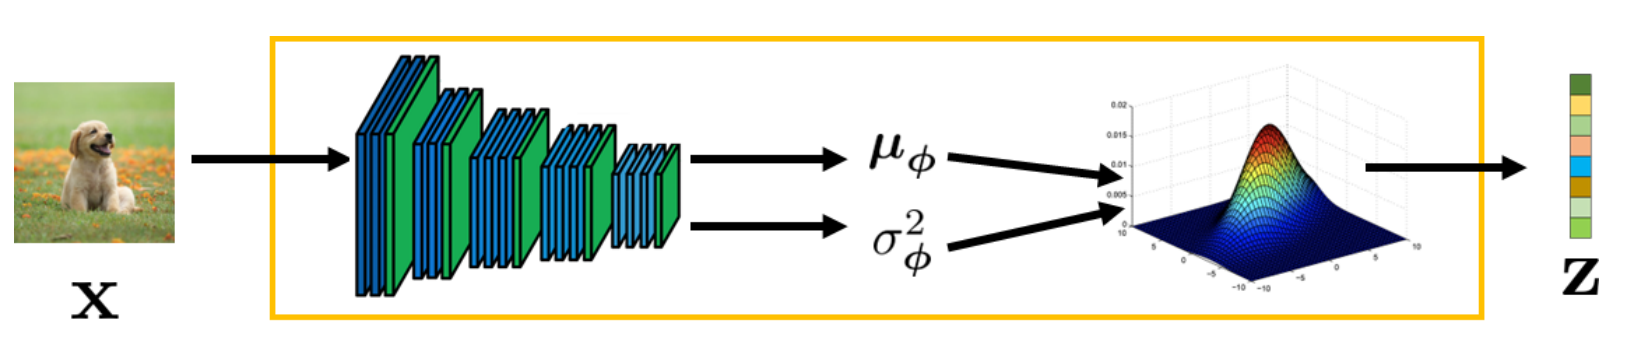
\includegraphics[width=0.7\linewidth]{figs/vae-encoder}
	\end{figure}
	\begin{figure}[h]
		\centering
		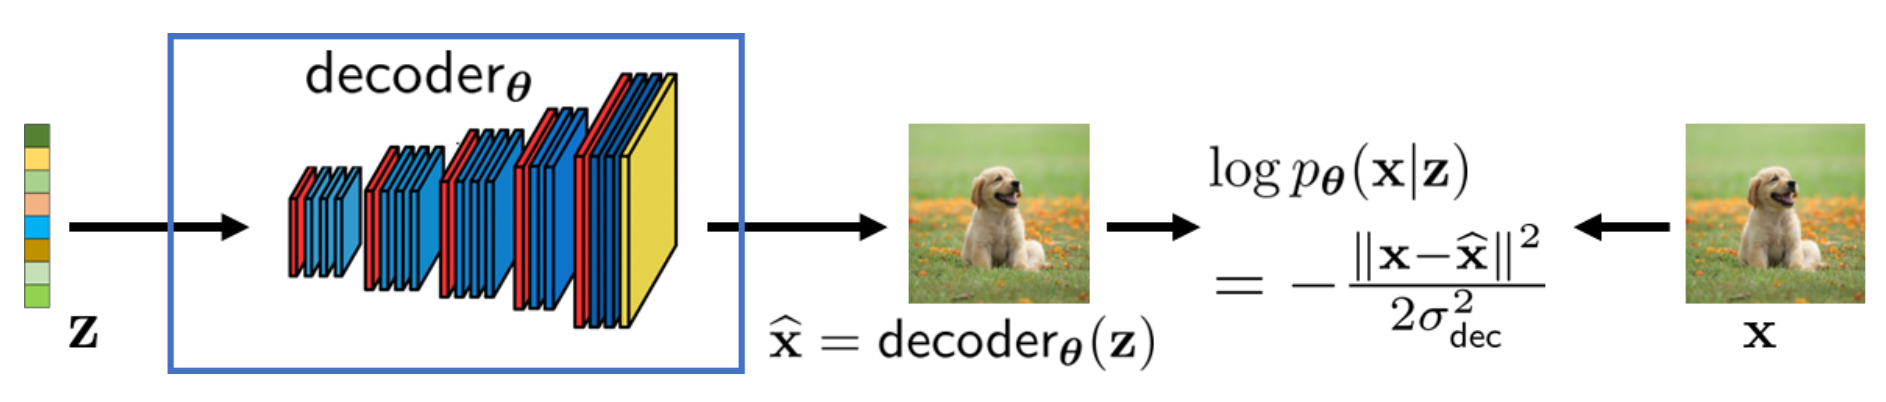
\includegraphics[width=0.9\linewidth]{figs/vae-decoder}
	\end{figure}
\end{frame}
%=======
\begin{frame}{Summary}
	\begin{itemize}
		\item NF models can be interpreted as VAEs with deterministic encoder and decoder functions.
		\vfill
		\item Discrete VAE latents offer a natural class of latent variable models.
	\end{itemize}
\end{frame}
%=======
\end{document}